\section{Introduction}
\begin{quotation}
\textit{Imagine an earthquake has hit a populous area and many major roads are
impassable. Buildings are serverly damaged or collapsed, and fire has broken out
in many places. At the crisis management center, response professionals are
working together to coordinate the earthquake relief effort. You are the
incident commander charged with coordinating the search
and rescue teams working in the field. There is a large tabletop display in
front of you, showing the map of the site. Information coming from the field is
updated on the display in real-time.}

\textit{A report about a big explosion at a chemical plant comes in and you move
the map around, zoom in and rotate it to get a good view of the plant. On the
map, you see there is a group of unmanned vehicles nearby. After selecting them
on the map with your hand, you speak to the interface ``Go nearer to the
explosion site to gather more information,'' while tracing the route the
vehicles should take to avoid obstacles. Then you instruct rescue team No. 3 to evacuate the residents
in the sorrounding buildings by going under a bridge because the surface of the
bridge is blocked. You gesture with one hand as the bridge and the other
hand moving under it to emphasize this.}
\end{quotation}

The scenario above shows an application of a multi-modal interface to a
real-world problem. Gestures play an important part in this scenario,
providing key information about location, method and timing of movements,
and about spatial relationship among the objects being described.

Recent trends in user interfaces have brought on a new wave of interaction
techniques that depart from the traditional mouse and keyboard that have been 
used for decades. These include multi-touch interfaces such as the 
iPhone\textsuperscript{\textregistered}, iPad and the Microsoft 
Surface\textsuperscript{\textregistered} as well as camera-based systems such as
the Microsoft Kinect and the Nintendo\textsuperscript{\textregistered} Wii. Most
of these devices gained instant popularity among consumers, and the common trait
among them is that they make interacting with computation more natural and 
effortless. All these devices allow users to use their hands and/or body 
gestures to directly manipulate the virtual objects. It feels more natural this 
way because this is how we interact with our environment in everyday life.
 
Our goal is to take this aspiration to the next level by developing an
intelligent multimodal interface for natural interaction. By \textit{natural
interaction}, we mean the kind of cognitively transparent, effortless multimodal
communication that can happen between people; we want to make this possible in
human-computer interaction such that the computer interface understands what the
user is saying and doing, and the user can simply behave. We believe that
natural interaction can provide better learnability, flexibility, memorability,
convenience and efficiency, but further user studies are needed to investigate
this belief.

Gesture plays an important part in multimodal interaction, especially for
conveying spatial information. The focus of this thesis is developing a
hierarchical approach for continous gesture analysis that can be easily
applied in different domains and applications. Specifically, we focus on
gestures made with hands.

\section{Background}
In thier review of visual interpretation of hand gestures for HCI, Pavlovic
\cite{Pavlovic97} et al. states that hand gestures in natural environments are
used for both manipulative actions and communication. However, the communicative
role of gestures is subtle, since hand gestures tend to be a supportive element 
of speech (with the exception of deictic gestures, which play a major role in 
human communication).

\section{Related Work}
There are many active research on using hand as an input modality for
human-computer interaction. To do this, the computer needs to be able to
interpret the dynamic and/or static configurations of the human hand, arm, and
even other parts fo the human body. (Mention Kettebekov's paper and the
framework. Gesture definition.)

\subsection{Sensors}
The first step in the pipeline is having sensors that captures the hand movement
and configurations, converting analog signals to digital signals. First attemps
to solve this problem resulted in mechanical devices that directly measure hand
joint angles and spatial position. This group is best represented by the
glove-based approaches using divecs such us CyberGloves \cite{fels09} and
Powergloves \cite{kadous02}. However, wearing gloves makes gesturing more
combersome and many efforts have been to make the gloves more light-weight by
using bluetooth wireless data transmission (e.g. CyberGove II). To further
reduce the bulkyness of the gloves, people use colored markers on the fingers
\cite{mistry09} or colored gloves with not electronics \cite{Wang09} and use RGB
cameras and computer vision techniques to interpret gestures. However, by
requiring the user wearing something additional still hinders the acceptance of
such device as a ``everyday'' natural interaction interface. 

The most nonobtrusive way to capture the hand is bare-hand tracking. People have
used different types of camera to achive this task. \cite{Shin04} used stereo RGB
cameras to extract the hand from background based on the skin color. One
limitation of use RGB cameras is they are very sensitive to lighting conditions.
This prompted researchers to look into other types of cameras. Oka et al. 
\cite{Oka02} uses thermal imaging for hand segmentation under compplex
background and changing light, relying on the condition that a hand's
temperature is almost always distince from the background. Their approach does
not detect finger contact with the surface. Larson et al. \cite{larson11}
improves on this method to detect the finger contact by using
the heat transferred from a user's hand to the surface for touch-based gestures.
However, inorder to detect the head trace, the user has to drag the fingers a
bit instead of just touching. This may be a small departure from what the user
would expect as ``natural'' based on the experience in the physical world.

Thermal imaging measures radiation emitted by objects in the F-IR spectrum.
There are other well-known ``IR-imaging'' techniques used in the HCI community
which use device that operate in the \textit{near}-infrared (N-IR) spectrum.
N-IR is employed in some fairly recent interactive tabletop surfaces and depth
cameras. A number of project in the HCI community have used IR for tabletop
interaction by detecting multi-touch gestures using an under mounted
camera and illumination source. An exmaple of this is Microsoft's 
Surface\textsuperscript{\textregistered}. Recently portable multi-touch devices
such as phones and tablets have become more and more ubiquitous. These devices
are based on capacitve touch sensitive screens. Touch-based devices are becoming
more and more mature, however the kind of gestures one can use are still
limited. The gestures are usually limited in 2D space with one or multiple
fingers. 

Going beyond the limitation of touch-only gesture, researchers at Microsoft
augmented the Surface technology with a switchable diffuser, additional
strips of IR LEDS with a different wave length for diffuse illumination, and an
additional IR sensitive camera which images IR reflected from the diffuse
illumination of the environment \cite{hilliges09}. In this way, they can capture
the hand above the surface as well. The height of the hand is estimated based on
the pixel intensity.

Since the introduction of Kinect, a motion sensing inut device by Microsoft for
the Xbox 360 video game console, researchers in the HCI community, as well as
many independent hackers, have been using Kinect's depth sensor for capturing
both body and hand gestures \cite{openni}. Since then, there are also many
similar devices coming into the market which have been used for capturing
gestures. For instance, Harrison et al. \cite{harrison11} uses  a short-range
PrimeSense \cite{primesense} depth camera for their wearable multitouch
interaction. In comparison to the aforementioned augmented Surface setup,
Kinect, and the likes, provides a cheap alternative for depth sensing. In this
thesis, we will explore the potential of using the Kinect sensor for detecting 
both the touch-based gesture and above-surface 3D gestures. Potentially, we can 
use the depth information for determing surface touch, and hence, eliminate the 
need for the complicated electronics of a touch sensitive screen. This also 
enables the gestural interaction on a large tabletop display, much bigger than 
that of Microsoft's Surface.

\subsection{Hand tracking}
After getting input from the sensor(s), the next step in the pipeline is
tracking the hand(s). This is essentially the frame-by-frame estimation of the
parameters of the hand model based on the sensor input. The complexity of the
hand model is application dependent. For a given application, a very coarse and
simple model may be sufficient. The simplest model is treating the hand as a
blob and only the 2D/3D location of the blob is tracked. For example, Sharma et
al. \cite{sharma00} used 2D positional and time differential parameters to track
the hands as blobs which was sufficient for them to distinguish whether the
hands were doing a point, contour or circle gesture. PrimeSense NITE requires the user to do a ``focus'' gesture (``click'' or
``wave'') to gain control and start hand-tracking \cite{primesense-manual}. The
gestures it supports are ``click'', ``wave'', ``swipe left'', ``swipe right'',
``raise hand candidate'' and ``hand candidate moved''.

However, to make a more generalizable system for natural-like interaction, a
more sophisticated model is required. One step forward is adding fingertips
location in the hand model as exmplified in \cite{Oka02} \cite{harrison11}
\cite{larson11}. Tracking fingertips is usually sufficient for manipulating
objects on the 2D surface. However, for a more rich set of gestures, the one
that also involves communicative gestures, we may need a more sophisticated
model. Wang et al. \cite{Wang09} uses a 26 degree of freedom (DOF) 3-D skeletal
model in their real-time hand-tracking system. 

Another approach is using appearance-based model. This means that the model
parameters are not directly derived from the 3D spatial description of the hand.
The gestures are modeled by relating the appearance of any gesture to the 
appearance of the set of predefined, template gestures \cite{Pavlovic97}. In
their markless hand tracking system, Wang et al. \cite{wang11} uses efficient
queries of a database of gesture and desktop-specific hand silhouette samples
for pinch/click gesture detection.

In our system, we propose a combination of both approaches. A 3-D skeletal hand
model is useful for manipulative gestures because we want to know exactly where
the fingertips are and the grabbing and releasing poses of the hand. For
communicative gestures, we just need to know the meaning of the gesture instead
of the exact spatial parameters. Hence a example template model would be more
suitable which may require less computation.

\subsection{Gesture recognition}
Most of the gestural input applications have been focusing on tracking only
\cite{harrison11} \cite{larson11}. For hand gesture recognition, much of the
work is on sythetic gestures, most notably sign language recognition
\cite{Bauer00} \cite{kadous02}. Wang et al. \cite{Wang09} made a simple
demonstration fo sign language finger spelling with their color glove hand-tracking system. 
For dynamic gesture recognition, hidden markov model (HMM) is a commonly used
technique because it is suitable for time series data \cite{sharma00}. 

Wang et al. \cite{wang06} argued that a significant limitation of the
HMM is the requirement of conditional independence of observations. In
addition, HMM, as a generative model, optimizes the likehood of
generating all the examples of a given gesture class, which is not
necessarily optimal for discriminating the gesture class against other
gestures. They introduced the use of hidden conditional random fields (HCRF) for
gesture recognition, and and showed improved accuracy for the set of head and
arm gestures they use compared with using HMMs. 

On the topic of discriminative vs. generative classifiers, Ng and Jordan
\cite{ng02} shows that while discriminative learning has lower asymptotic error,
a generative classifier may also approachy its higher asymptotic error much
faster. Their claim is based on experiments with the naive Bayes classifier and
logistic regression Generative-Discriminative pair. This means the performance
of the two kinds of classifiers may be dependent on the number of training
examples. In this thesis, we will compare both the HMM and HCRF approach and
analyze their performance based on the number of training examples.

There are few work that actually distinguishes manipulative gestures and
communcative gestures. Oka et al. \cite{Oka02} developed a system that allows
both direct manipulation and symbolic gestures. Based on the tracking result,
the system first differentiates the gesture as either manipulative or symbolic 
according to the extension of the thumb. They regard gestures with an extended 
thumb as direct manipulation and those with a bent thumb as symbolic gestures. 
For direnct manipulation, the system selects operating modes such as rotate, 
move or resize based on the fingertips configuration; for symbolic gestures, it 
uses HMM for classification. The way they distinguish manipulative and 
communicative gestures seems to be arbitrary and ``unnatural''. They did that 
probably for the ease of it because they are only trakcing fingertips.

We propose an interface that can seamlessly switching between between
manipulative and communcative gestures based on the learned parameters. We
believe the distinction among different classes of getures is useful for the
input system because the best parameter space may be different for different
classes. This motivate our hierachical approach to continuous gesture
recognition.

\subsection{Multimodal systems}
Bolt's pioneering work in the ``Put That There'' system \cite{Bolt80} 
demonstrated the potential for voice and gestural interaction.  In that system, 
the hand position and orientation was tracked by the Polhemus tracker, i.e., the
hand was essentially transformed to a point on the screening. The actual hand 
posture did not matter, even if it was not in a pointing shape. The speech also 
followed a rigid and limited command-like grammar. Even though this is an early 
work, it provides some insight about the advantages of multimodal interaction. 
As Bolt summarized in the paper, using pointing gesture allows the use of 
pronouns in the speech, with the corresponding gain in naturalness and economy 
of expression \cite{Bolt80}.

Since then, several multi-modal interaction prototypes were 
developed that moved beyond Bolt's ``Put That There'' system. Cohen et al. 
\cite{Cohen97} developed the QuickSet prototype which is a collaborative, 
multimodal system running on a hand-held PC using pen and voice as input. They 
used a novel multimodal integration strategy that allows speech and pen gesture 
to compensate for each other, yielding a more robust system. Rauschert et al. 
\cite{Rauschert02} developed a system called Dialogue-Assisted Visual 
Environment for Geoinformation (DAVE\_G) that uses free hand gestures and speech
as input. They recognized that gestures are more useful for expressing spatial 
relations and locations. Gestures in DAVE\_G included pointing, indicating an 
area and outlining contours. Speech and gesture are fused for commands that need
spatial information provided by the gesture. 

In this thesis, we will also explore the fusion of speech gestures. In addition
to use the deicitc gestures to provide spatial information as a complement to
speech as in \cite{Rauschert02}, we will also explore the the use of speech as a
complement to manipulative gestures based on the finding from a user study done
by Yin et al.\cite{yin10}. They observed that manipulative gestures are at times
accompanied by adjectives and adverbs that refine the actions.

\section{Proposed Work and Procedure}
Our long term goal is to build an intelligent multimodal interface for natural
interaction that can serve as a testbed for enabling the formulation of a more
principled system design framework for multimodal HCI. One focus of this thesis
is on the gestural input modality. The user should be able to use gesture as an
input effortlessly for both direct manipulation and communication to the system.

\subsection{Gestural Taxonomy}
We adopt the taxonomy of hand movements proposed by Pavlovi\'{c} et al.
\cite{Pavlovic97} which distinguishes gestures from unintentional hand movements
(like beats). They then further divided the gestures into manipulative and 
communicative classes. 

Manipulative gestures are the ones used to act on objects, while communicative 
ones have an inherent communicational purpose\cite{Pavlovic97}. For manipulative
gestures, the system needs to repond frame by frame while the user is doing
certain direct manipulations. This part is related to tracking of the hand
state. For communicative gestures, the system needs to repond to the meaning of
the gesture when the user finishes performing the gesture. This part is
accomplished by the gesture recognizer.

\subsection{System Setup}
The custom tabletop structure includes four $1280\times1024$ pixel projectors 
(Dell 5100MP) that provide a $2560\times2048$ pixel resolution. The display is 
projected onto a flat white surface digitizer (GTCO Calcomp DrawingBoard V), 
which uses a stylus as an input device. The digitizer is tilted 10 degrees down 
in front, and is placed at 41in (104cm) above the floor, following FAA's design 
standard to accommodate the $5^{th}$ through $95^{th}$ percentiles of 
population. Projected displays were mechanically aligned to produce a single 
seamless large display area.

\begin{figure}
  \centering
  \subfigure[] {
	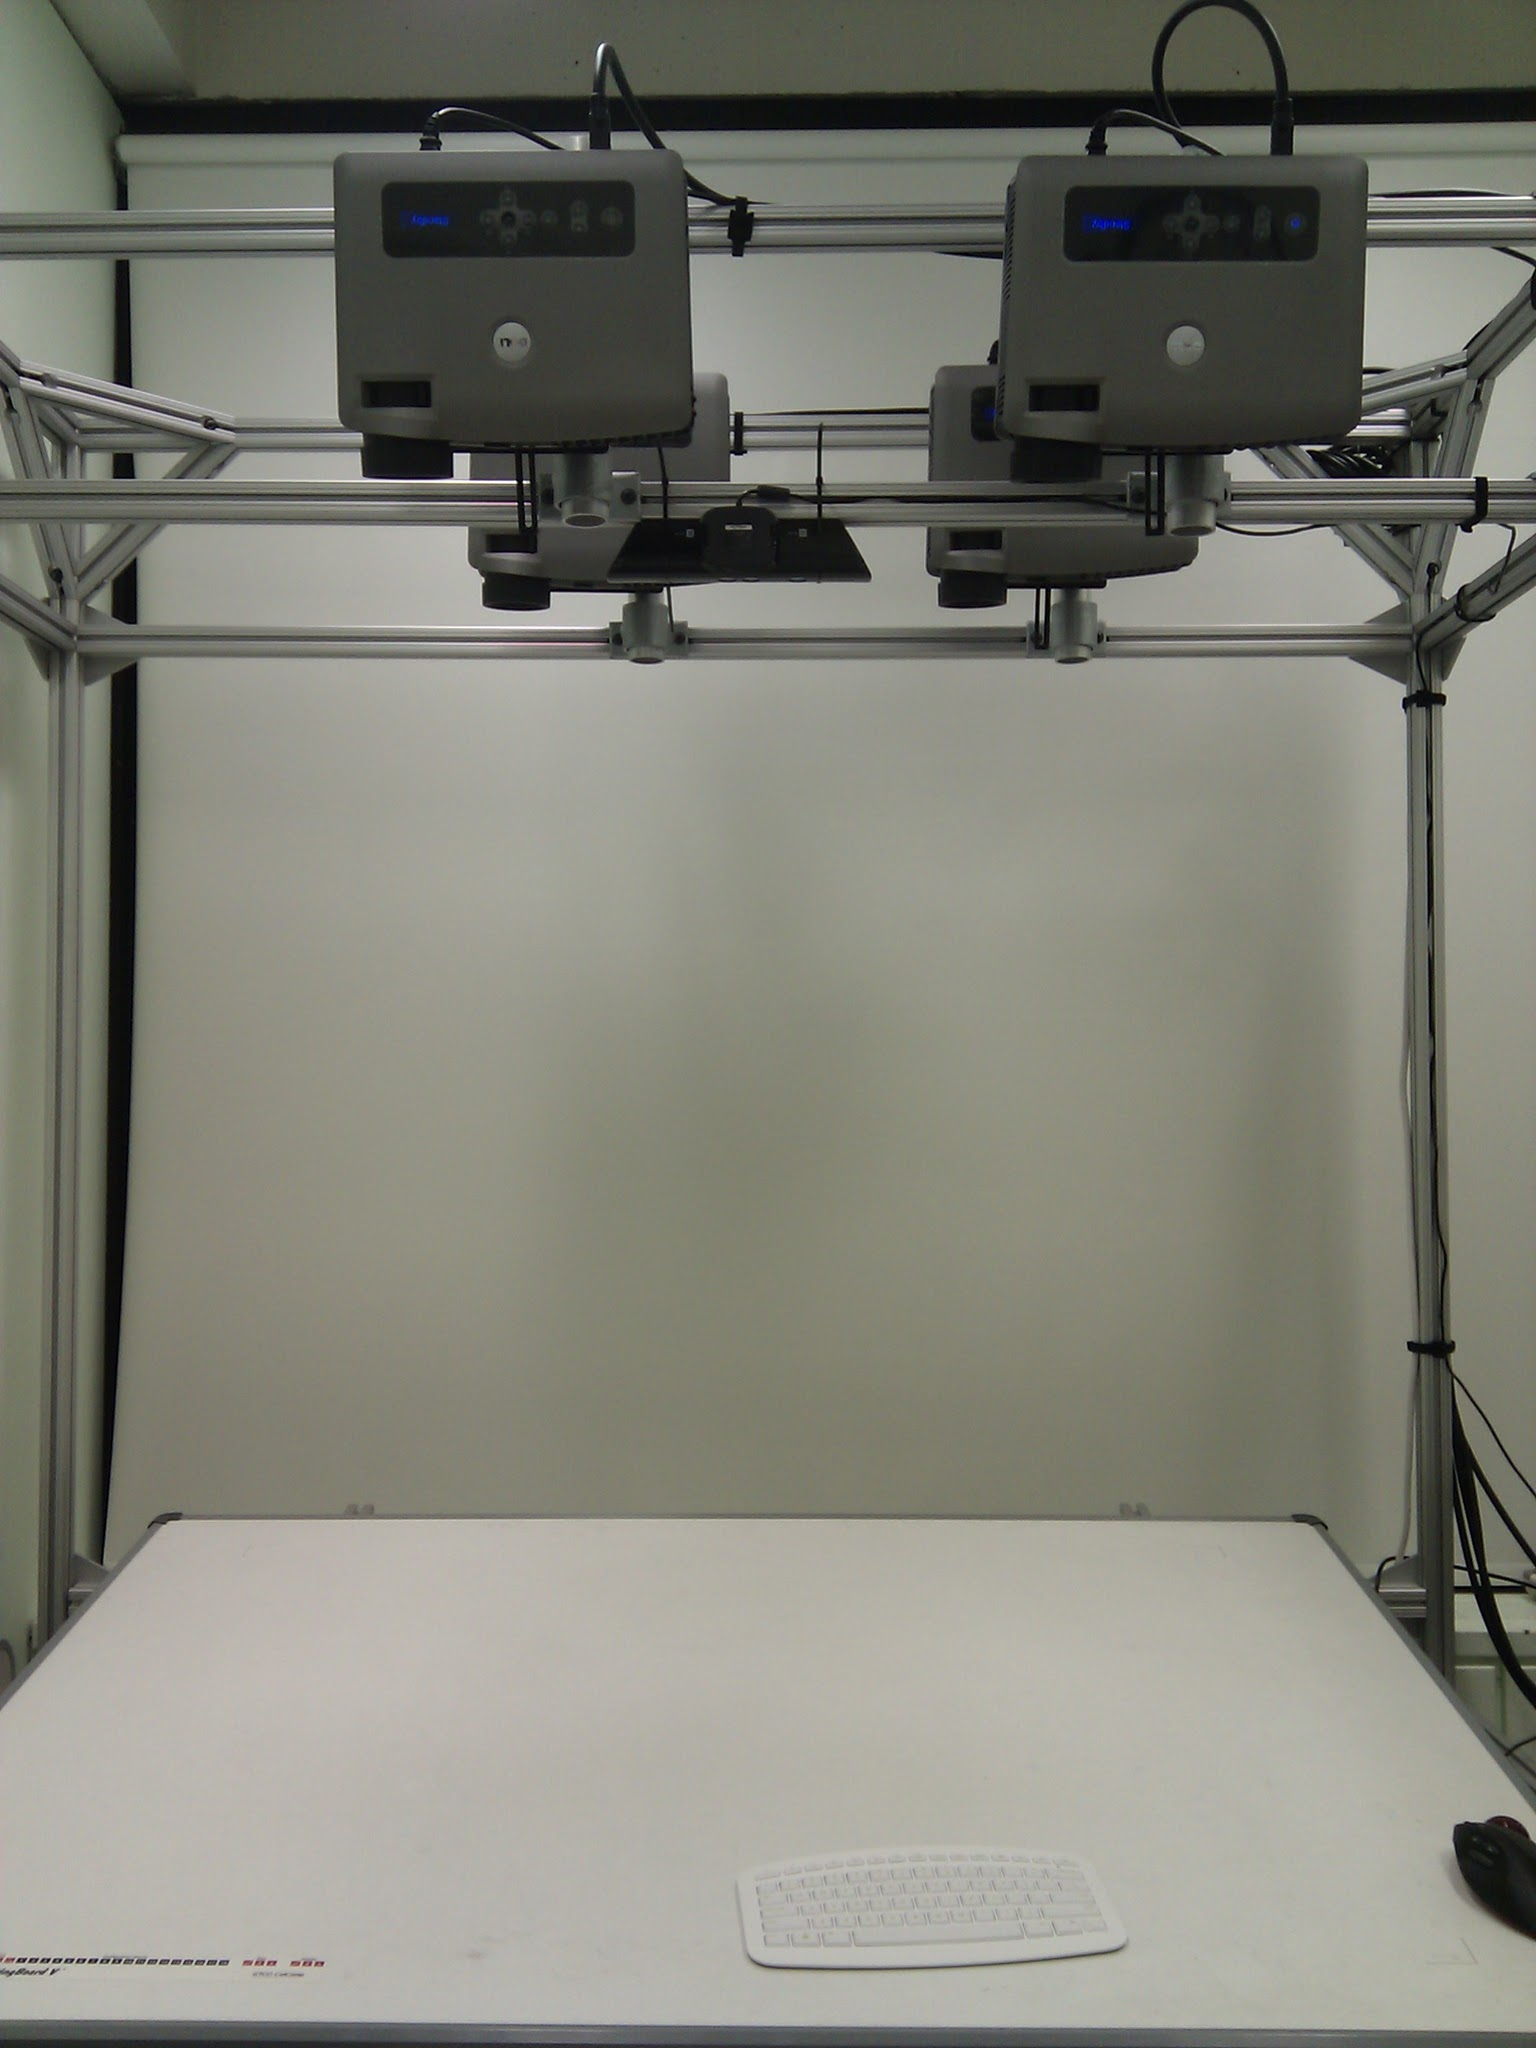
\includegraphics[width=0.4\textwidth]{figures/setup1.png} 
  }
  \subfigure[] {
  	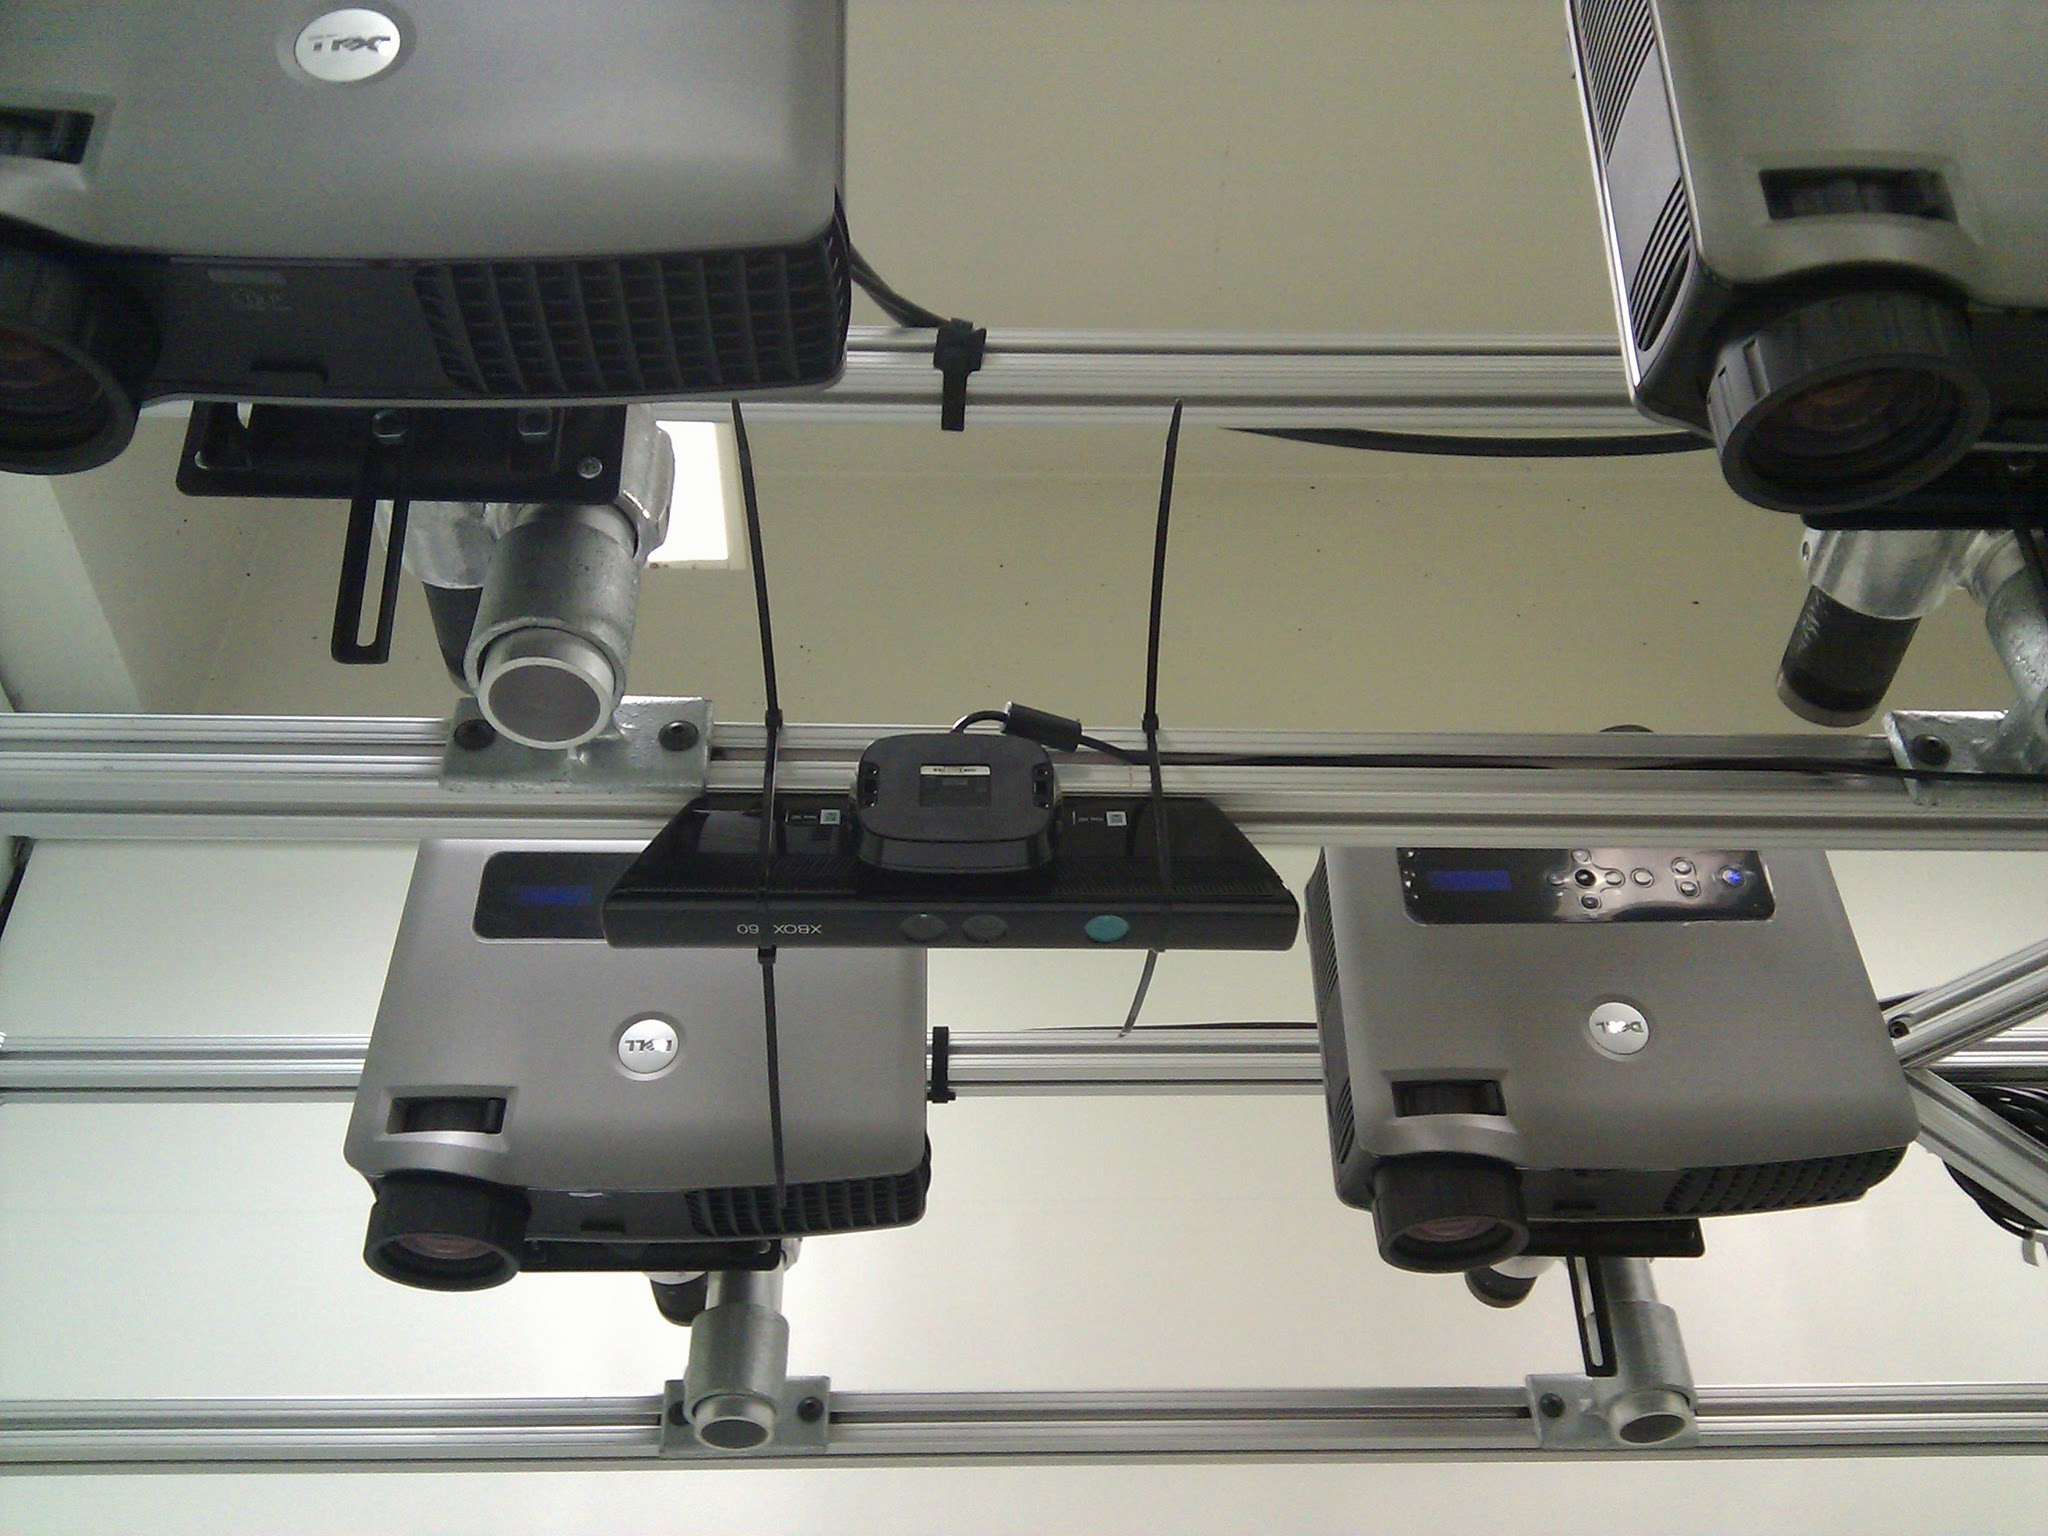
\includegraphics[width=0.4\textwidth]{figures/setup_close.png}
  }
  \caption{System setup.} \label{fig:setup}
\end{figure}

One Kinect motion sensor by Microsoft is placed above the center of the tabletop
at the same level of the projectors. Figure~\ref{fig:setup} shows the setup. The
Kinect sensor has a RGB camera, a depth sensor and a multip-array microphone. We
are using the depth sensor for capturing the hand motion data because it is less
sensitive to the lighting condition. This is particularly useful for our
projection system. The Dell 5100MP projector uses a spinning color wheel to
modulate the image. This produces a visible artifact on the screen, referred to 
as the ``rainbow effect'', with colors separating out in distinct red, green, 
and blue. At any given instant in time, the image on the screen is either red, or green, or blue,
and the technology relies upon people's eyes not being able to detect the rapid 
changes from one to the other. However, when seen through a camera, the effect 
is very obvious, and this can greatly affect hand segmentation if we were to use 
the RGB images. 

The Kinect sensor output video at a frame rate of 30Hz. The depth sensing video
stream has a resolution of $640\times 480$ pixels with 11-bit depth value. The
depth value increases as the distance of the object from the sensor increases.
The depth sensor has a range limit of about 0.5m - 5m with a resolution of 1.5mm
at 0.5m and 5cm at 5m. The tabletop surface is about 1.2m away from the Kinect
sensor which allows us to have a relatively good depth resolution. We use the
open source OpenNI framework \footnote{https://github.com/OpenNI/OpenNI} and its
Kinect driver \footnote{https://github.com/avin2/SensorKinect} to get both the depth and RGB data streams.

\subsection{Kinect Calibration}
In order to develop the interactive interface, we need to map the point in the
depth data frame to the point on the display. We do this by projecting a
checkerboard image on the tabletop display, and placing some wooden blocks at
the corners of the checkerboard image to create the depth differences so that 
the depth sensor can capture these corners (see Figure~\ref{fig:calibration}).
We manually labeled 16 pairs of corresponding points on the display and in the depth image data frame. Then we
apply undistortion and planar homography to find the mapping.

\begin{figure}[h]
  \centering
  
\includegraphics[width=0.5\textwidth]{figures/calibration.png} 
  \caption{Kinect calibration. The darker squares are the wooden blocks. The
  intensity of gray level image is inversely proportional to the distance from
  the Kinect sensor.}
  \label{fig:calibration}
\end{figure}

Planar homography is a projective mapping from one plane to another. In our
case, we are mapping points in the plane of the depth image frame to the points
on the plane of the display.

\subsection{Hand Tracking}
The hand tracking pipeline consists the following steps:

\begin{enumerate}
  \item Background subtraction
  \item Forelimb and hand segmentation
  \item Fingertips tracking
\end{enumerate}

The following subsections explain in details about these steps. Many of the
computer vision methods we use are based on the OpenCV
\footnote{http://opencv.willowgarage.com/wiki/} library and the Java interface JavaCV \footnote{http://code.google.com/p/javacv/}.

\subsubsection{Background Subtraction}
The background which is the tabletop is relatively static, but there are still 
noises from the depth sensor. We use the averaging background method which
learns the average and average difference of each pixel as the model of the 
background based on the initial 30 frames with no hands in the scene. For the
subsequent frames, any value that is 6 times the average frame-to-frame absolute
difference below the average tabletop depth value for that pixel is considered 
foreground because it's closer to the sensor above.

To clean up the background subtracted depth image, we use 1 iteraction of
morphological opening to clear out small pixel noise. Morphological opening is a
combination of erosion and dilation. Both erosion and dilation are morphological
transformations. The kernel of erosion is a \textit{local minimum} operator,
while that of dilation is a \textit{local maximum} operator.

\subsubsection{Forelimb and hand segmentation}
With the cleaned up background subtracted depth image, we find connected
components by finding all contours that are not too small. These components are
considered to be the forelimbs and are approximated with convex hulls and 
bounding boxes. The hand region is at either end of the bounding box.

\subsubsection{Fingertips Tracking}
We base our estimation of the hand model on the geometric property of the
hand. We compute the convexity defects from the convex hull of the forelimb.
From this we can observe that for an extended finger, it has one convexity
defect on each side and the the two adjacent sides of the the defects form an
acute angle. We iterate through the adjacent convexity defects, and mark the
intersection of those sides that forms an angle that is smaller than a threshold
value as the potential fingertip. We further refine the fingertip position by
searching in the general direction of the finger and find the sharp change in
the gradient of the depth value.

\subsubsection{Kalman Filter}
We use Kalman filter to further improve the tracking accuracy. We use a
$4$-dimentional vector, including x, y coordinates and the velocity in x, y
coordinates of the fingertip, as the dynamic state of the fingertip.
The measurement is a $2$-dimensional vector of the measured x, y
coordinates of the fingertip. 

Assuming no external control, the a priori estimate $x_k^-$ of the state is
given by:
\begin{align*}
x_k^- = Fx_{k - 1} + w_k,
\end{align*}
where $F$ is the $4$-by-$4$ \textit{transfer matrix} characterizing the
dynamics of the system with the following values

\begin{align*}
F = \left[ \begin{array}{cccc}
	1 & 0 & 1 & 0 \\
	0 & 1 & 0 & 1 \\
	0 & 0 & 1 & 0 \\
	0 & 0 & 0 & 1 \end{array} \right],
\end{align*}

and $w_k$ is the
\textit{process noise} associated with random events or forces that directly affect the actual state of the system. We assume that the components of $w_k$
have Gaussian distribution $N(0, Q_k)$ for some $4$-by-$4$ covariance matrix
$Q_k$.

Using $P_k^-$ to denote the error covariance, then a priori estimate for this
covariance at time $k$ is obtained from the value at time $k - 1$ by:
\begin{align*}
P_k^- = FP_{k - 1}F^T + Q_{k - 1}
\end{align*}

We set the matrix Q with the following values:
\begin{align*}
Q = \left[ \begin{array}{cccc}
	1 & 0 & 0 & 0 \\
	0 & 1 & 0 & 0 \\
	0 & 0 & 10 & 0 \\
	0 & 0 & 0 & 10 \end{array} \right],
\end{align*}
   
\subsection{Gesture Recognition}
We propose ot use machine learning method to differentiate
manipulative gestures and communicative gestures. For manipulative gesture, if
we only consider touch gesture as manipulative, we only need to find the points
where the depth of the hand is close to the table surface. If we also want to
allow non-touch based manipulative gesture, we need to use the simplied hand
skeletal model from hand-tracking. 

Gesture recognition is used for communicative
gesturs. We will bootstrap the system with gesture models learned from users.

We propose to compare the result between using hidden conditional random field
and HMM for the continuous gesture recognition. We want the system to be able to
learn from a relatively small number of training examples for each gesture, so
that the user can easily define their own gestures. With a small number of the
training examples, it is not clear that the discriminative model of HCRF will
perform better than HMM. 

(Continuous gesture)

\subsection{Communicative Gesture and Speech Recognition} 
For this study, we will focus more on gestural input and interaction. 
However, we may add some basic speech recognition capability to the system in order to combine speech and
deictic gestures for some USAR interaction scenarios.

\subsection{Motivating Application}
We will develop a simple game-like application that simulates some of the USAR
interaction scenarios.

\subsection{User Study}\label{sec:userStudy}
Following the exploratory user study done by Yin et al. \cite{yin10}, we will
conduct a user study after making the simple appplication where the user can 

\section{Schedule}
% \begin{enumerate}
% 	\item Experiment with polarizing filters \hfill Done by Jan 31, 2010
% 	
% 	Test whether using polarizing filters can provide better result than computing the background, or maybe we can use both methods.
% 	
% 	\item Continuous online gesture recognition \hfill Done by Feb 14, 2010
% 	
% 	Improve algorithms on continuous online gesture recognition. Conduct quantitative evaluation of the recognition results. 
% 	
% 	\item Connect user interface with gesture recognition	\hfill Done by Feb 28, 2010
% 	
% 	Interface with Google Earth. Improve system response time with gesture interaction. May need to switch to more rudimentary map interface if speed is an issue for Google Earth. May add basic speech recognition.
% 	 
% 	\item User study \hfill Done by Mar 21, 2010
% 	
% 	Conduct user study described in Section \ref{sec:userStudy}.
% 	
% 	\item Write first draft of thesis report \hfill Done by Apr 15, 2010
% 	\item Complete thesis report	\hfill Done by Apr 30, 2010
% 	\end{enumerate}
% 	
\section{Principal Equipment and Facilities}
Here is a list of equipment and facilities needed for the study:

\begin{enumerate}
	\item A white surface digitizer (GTCO Calcomp DrawingBoard V)
	\item Four $1280\times1024$ pixel projectors (Dell 5100MP)
	\item One Kinect motion sensor
	\item One desktop with powerful graphics card
\end{enumerate}

All the above equipment are avalaible.

\section{Appendix A - Kalman Filter}
Let $x_k$ be an $n$-dimentional vector of state components and $P_k$ be the
$n$-by-$n$ error covariance. The measurements $z_k$ is a $m$-dimensional
vector given by:
\begin{align*}
z_k = H_kx_k + v_k,
\end{align*}
where $H_k$ is an $m$-by-$n$ matrix and $v_k$ is the measurement error.

The \textit{Kalman gain}, $K_k$, is an $n$-by-$m$ matrix expressed as:
\begin{align*}
K_k = P_k^-H_k^T(H_kP_k^-H_k^T + R_k)^{-1}
\end{align*}

Assuming no external control, the a priori estimate $x_k^-$ of the state is
given by:
\begin{align*}
x_k^- = Fx_{k - 1} + w_k,
\end{align*}
where $F$ is the $n$-by-$n$ \textit{transfer matrix} characterizing the
dynamics of the system, and $w_k$ is the \textit{process noise} associated with
random events or forces that directly affect the actual state of the system. We assume that the components of $w_k$
have Gaussian distribution $N(0, Q_k)$ for some $n$-by-$n$ covariance matrix
$Q_k$.

Using $P_k^-$ to denote the error covariance, the a priori estimate for this
covariance at time $k$ is obtained from the value at time $k - 1$ by:
\begin{align*}
P_k^- = FP_{k - 1}F^T + Q_{k - 1}
\end{align*}

The updated value for $x_k$ when a new measurement is available is:
\begin{align*}
x_k = x_k^- + K_k(z_k^- - H_kx_k^-)
\end{align*}
The update value for $P_k$ is:
\begin{align*}
P_k = (I - K_kH_k)P_k^-
\end{align*}
